% Created 2017-07-12 Wed 00:00
\documentclass[presentation]{beamer}
\usepackage[utf8x]{inputenc}
\usepackage[T1]{fontenc}
\usepackage{fixltx2e}
\usepackage{graphicx}
\usepackage{longtable}
\usepackage{float}
\usepackage{wrapfig}
\usepackage{rotating}
\usepackage[normalem]{ulem}
\usepackage{amsmath}
\usepackage{textcomp}
\usepackage{marvosym}
\usepackage{wasysym}
\usepackage{amssymb}
\usepackage{hyperref}
\tolerance=1000
\usepackage{minted}
\usetheme{metropolis}
\setbeamertemplate{frame footer}{Erwin Rooijakkers}
\metroset{block=fill}
\usetheme{default}
\author{Erwin Rooijakkers}
\date{12-07-2017}
\title{Blockchain, Ethereum, ClojureScript, Fleet}
\hypersetup{
  pdfkeywords={},
  pdfsubject={},
  pdfcreator={Emacs 25.1.1 (Org mode 8.2.10)}}
\begin{document}

\maketitle

\section{Blockchain}
\label{sec-1}

\begin{frame}[label=sec-1-1]{What?}
\begin{quotation}
"A \alert{shared}, programmable, cryptographically secure and therefore trusted ledger
\alert{which no single user controls} and \alert{which can be inspected by everyone}."

-- Klaus Schwab (Chairman World Economic Forum)
\end{quotation}
\end{frame}

\begin{frame}[label=sec-1-2]{Four pillars}
\begin{itemize}
\item Cryptographic Tokens and Addresses
\item P2P Networking
\item Consensus Formation Algorithm
\item Virtual Machine
\end{itemize}
\end{frame}

\begin{frame}[label=sec-1-3]{This.}
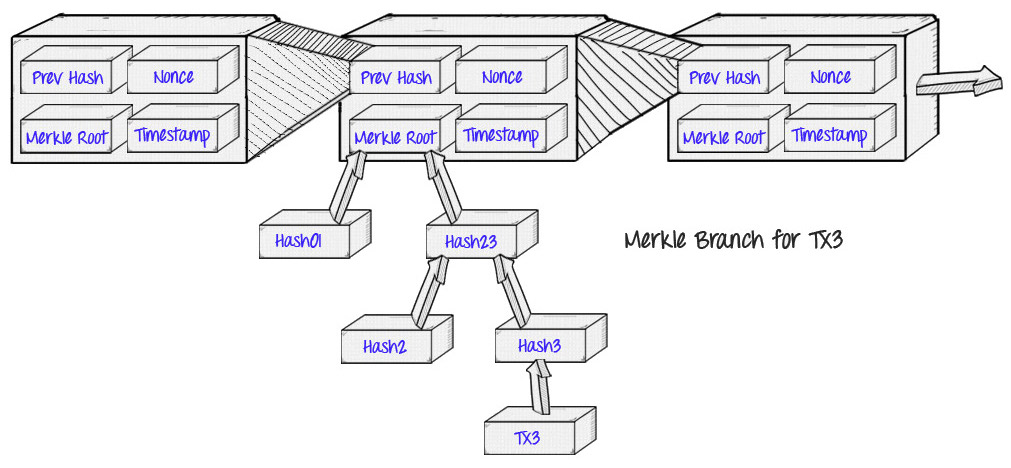
\includegraphics[width=.9\linewidth]{../images/merkle.jpg}

(Source: \url{https://blog.ethereum.org/2015/11/15/merkling-in-ethereum/})
\end{frame}

\begin{frame}[label=sec-1-4]{Consensus}
\begin{itemize}
\item \alert{Proof of Work (PoW)}: the current difficulty in the Bitcoin network requires
miners to try quadrillions of times before finding a nonce that fits.
(because \alert{hashing} can provide vastly different outputs on minor changes)
\item \alert{Proof of stake (PoS)}: mining is done by stakeholders in the ecosystem who
have the strongest incentives to be good stewards of the system. (E.g., by
setting coins aside for a longer period as stake.)
\end{itemize}
\end{frame}

\section{Smart Contracts}
\label{sec-2}

\begin{frame}[label=sec-2-1]{Model}
\begin{itemize}
\item Stateless webservices
\item Contract-oriented programming
\item Gas fees
\end{itemize}
\end{frame}

\begin{frame}[label=sec-2-2]{Stateless web services}
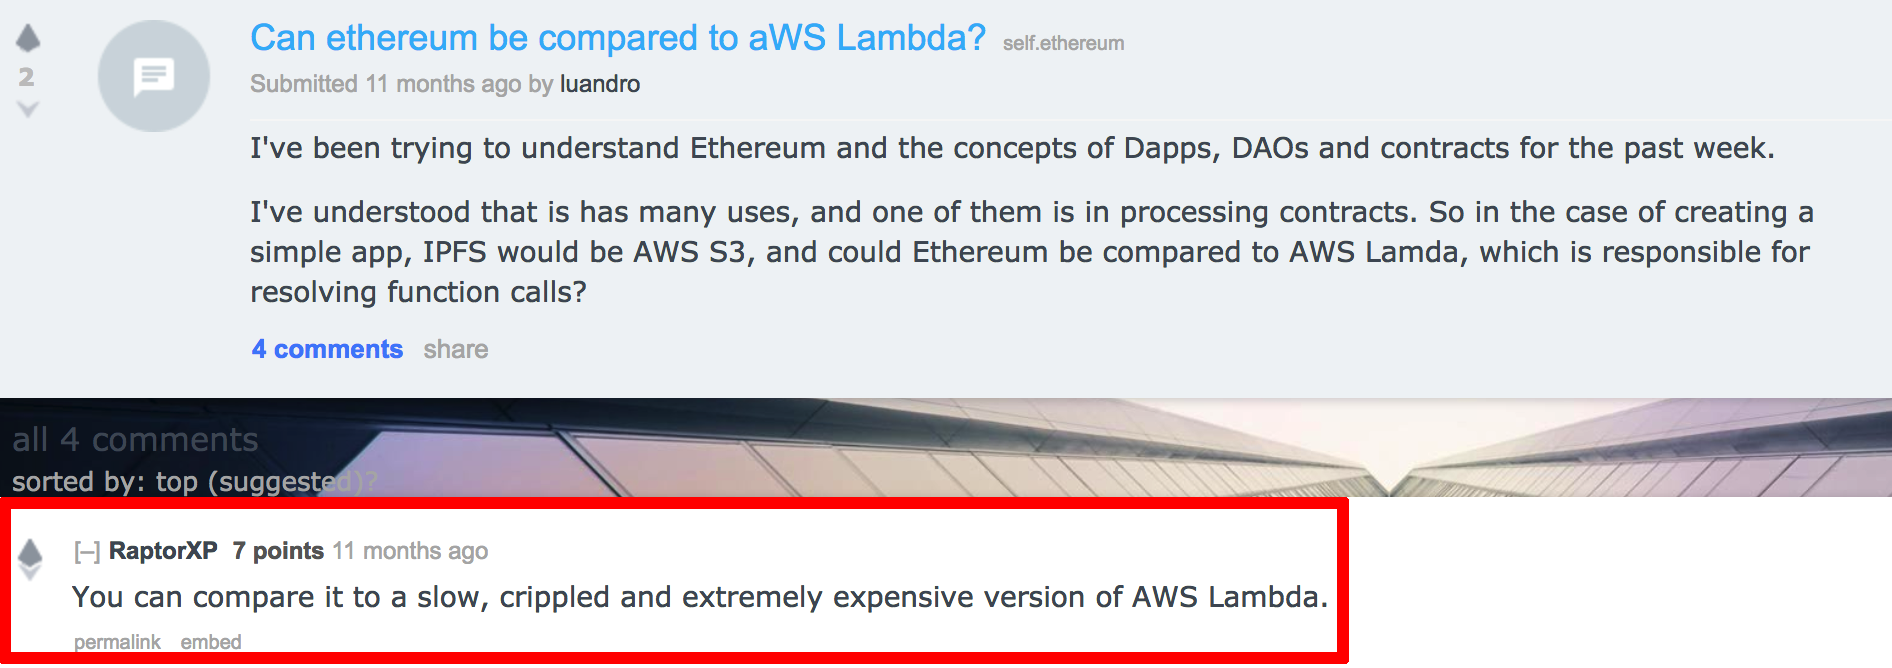
\includegraphics[width=.9\linewidth]{../images/awslambda.png}
\end{frame}

\begin{frame}[fragile,label=sec-2-3]{Contract-oriented programming}
 \begin{minted}[bgcolor=white,frame=lines]{javascript}
contract HelloSayerFactory {

  function create() returns (address) {
    return address(new HelloSayer());
  }

  function delete(address addr){
    HelloSayer(addr).remove();
  }

}
\end{minted}
\end{frame}

\begin{frame}[label=sec-2-4]{Tools}
\begin{itemize}
\item geth: (Go Ethereum) \alert{cli} for running full Ethereum node, exposes RPC
\item web3.js: Ethereum compatible \alert{JavaScript API} which implements the Generic \alert{JSON RPC spec}
\item solc: JavaScript bindings for Solidity compiler (creates \alert{ABI} and \alert{BIN})
\end{itemize}
\end{frame}

\begin{frame}[label=sec-2-5]{MetaMask (also: Mist; Parity)}

\includegraphics[width=.9\linewidth]{../images/metamask.png}
\end{frame}

\section{Fleet}
\label{sec-3}
\begin{frame}[label=sec-3-1]{Why ClojureScript + blockchain}
\begin{itemize}
\item \alert{Blockchain}
\item \alert{ClojureScript}!
\begin{itemize}
\item Reagent
\item Figwheel
\end{itemize}
\end{itemize}
\end{frame}

\begin{frame}[label=sec-3-2]{Code inspiration and big help}
\begin{itemize}
\item \url{https://medium.com/@matus.lestan}
\item \url{https://github.com/district0x/ethlance}
\item \url{https://ethlance.com/\#/job/128}
\end{itemize}

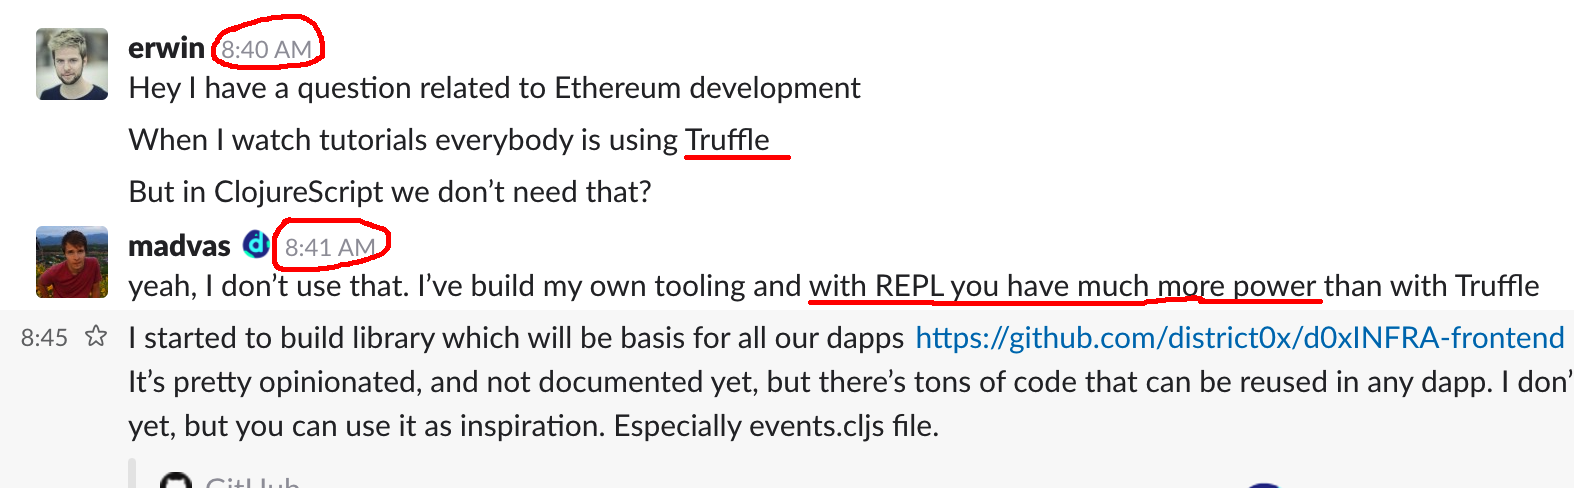
\includegraphics[width=.9\linewidth]{../images/madvas.png}
\end{frame}
\begin{frame}[label=sec-3-3]{Idea}
\begin{itemize}
\item Elisa Achterberg (Circle Economy and Sustainable Finance Lab) \emph{et al.}
\end{itemize}
\end{frame}

\begin{frame}[label=sec-3-4]{The idea}
\begin{itemize}
\item \alert{Linear economy} \emph{designs for failure} and sells \alert{“almost-broken” products},
creating \alert{waste}
\item When they are used, \alert{smart assets} (a \alert{\uline{fleet}} of assets) pay parties
involved in value chain (involved with design, commodities, creation,
maintenance, et cetera)
\begin{itemize}
\item Shift \alert{\emph{from ownership to use}} leads to \alert{Circular Economy}
\item \alert{A circular value network} in which materials and products are
shared as well as risks and returns
\end{itemize}
\end{itemize}
\end{frame}

\begin{frame}[label=sec-3-5]{Design}
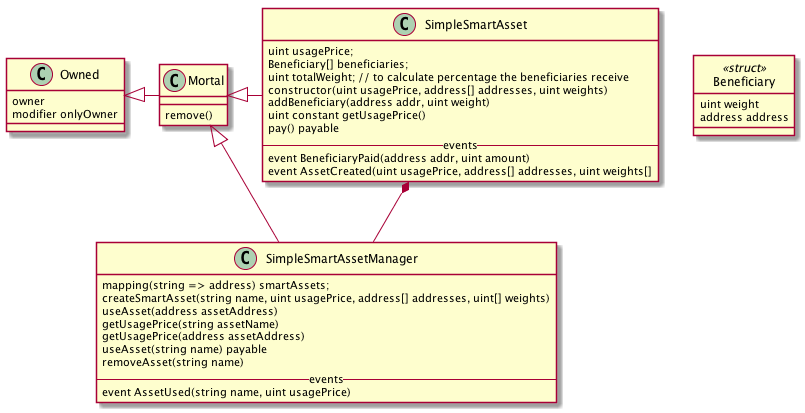
\includegraphics[width=.9\linewidth]{../images/fleet.png}
\end{frame}

\section{Fleet demo}
\label{sec-4}
% Emacs 25.1.1 (Org mode 8.2.10)
\end{document}
